% see A1.2
% see A3
% see B6.2b
\begin{landscape}
  \chapter{Zeitplan}
  Der Zeitplan basiert auf der Vorlage \cite{Buhler_ipa-timetable_2022} und zeigt mit einer Auflösung von zwei Stundenblöcken die geplanten und getätigten Aufwände.
  \begin{figure}[H]
    \begin{center}
      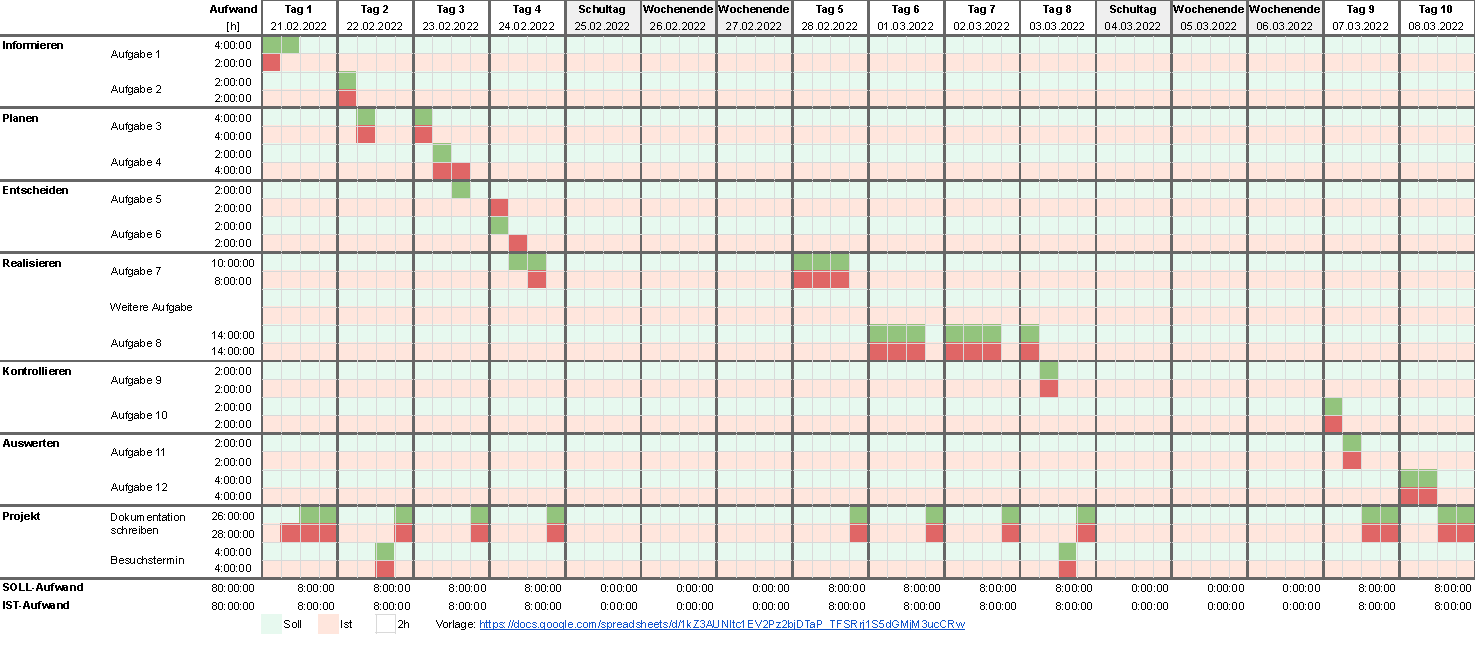
\includegraphics[width=1.55\textheight]{../res/timeplan.pdf}
    \end{center}
    \caption[\enquote{Zeitplan} erstellt mit Google Sheets]{Zeitplan}
    \label{fig:timeplan}
  \end{figure}
\end{landscape}
